\chapter*{Hexagonal Architecture}

The pattern we've just used, where we created an abstract interface for a connection between our system and the outside world, has a general name: a \emph{ports and adapters} architecture.

To understand where this name comes from, think about the display port on a laptop. You can plug in different adapters that let you connect your laptop to various types of displays - HDMI, DVI or even VGA.

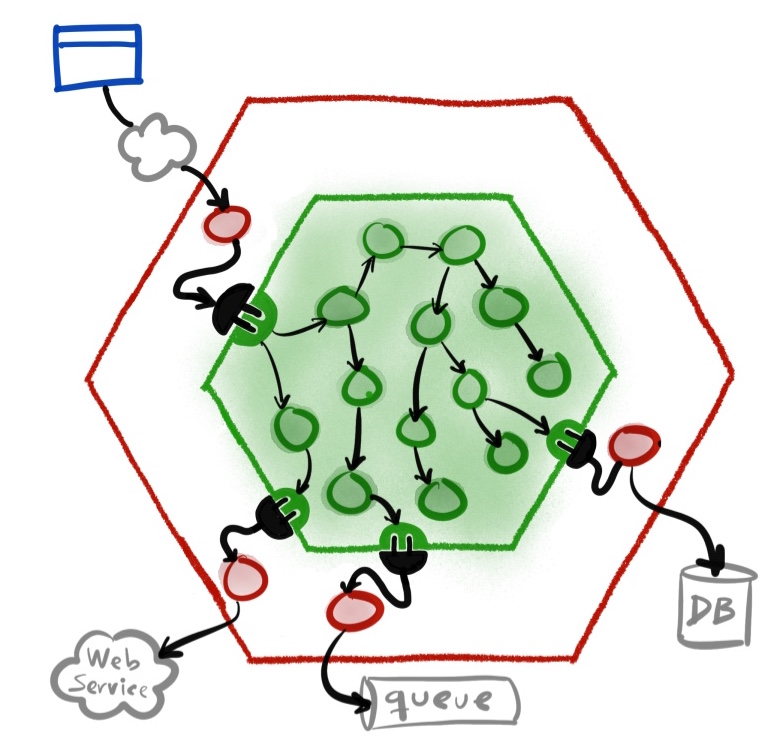
\includegraphics[width=\textwidth]{images/hexagonal-architecture}

In a ports and adapters architecture the core business logic is isolated from the technical infrastructure necessary to interact with the real world -- file systems, databases, message queues, user interfaces, transport protocols and so on. The application provides interfaces -- or \emph{ports} -- that define how it will communicate with the outside world. Different concrete implementations of these interfaces -- or \emph{adapters} -- encapsulate the application's interactions with an external service or system.

This is sometimes also known as a \emph{hexagonal architecture}\footnote{http://alistair.cockburn.us/Hexagonal+architecture}, mostly because that makes for a nice diagram!

This architecture not only makes your application code easier to reason about, it makes testing your core business logic much easier, because you can plug in testing infrastructure at the ports. For example, you can choose to use a fake, in-memory, database instead of a real one, or make API calls directly into a port to issue commands, rather than having to fire up a user-interface and push buttons on it.

As you've just seen, you can also test your adapters independently, meaning that all of your code is still covered by tests, but as few as possible of those tests are coupled to the slow, unstable reality of the outside world.


\section*{What does your hexagon look like?}

Think about the ShoutyReports batch job code as it stands right now. 

\QandAbox{Where are the ports? What adapters do we have?}{5}

We have two ports on our \texttt{\ShoutyReportProcessor}: one that takes in the mileage claims that were parsed from the CSV file, and another that communicates with the stats service.

\QandAbox{Draw a diagram like the one above for the ShoutyReports codebase.}{15}

